\section{Security}

Security is the way to support the privacy requirements, maintain control over the system, and assure data integrity.

\subsection{Physical Access Control}

As it was initially stated a significant part of the infrastructure is gonna be in public places. Thus we need to provision against security threads due to physical access on these machines; control nodes, guest nodes, and sensors. The event of a device theft should be considered as certain.

Our goals are: node breach isolation, attack impairment, attack repel, equipment tracking.

\subsubsection{Isolation}

One of the most important requirement in the design process should be that the breach/theft of a single node could not jeopardize the security of the remaining system. Things that are affected by this requirement are the existence of plain-text passwords, key-pairs for automatic authentication and login, and encryption keys.

Ideally no key pair co-exists at any of the publicly available systems, an exception to that rule is the public-private pair that is unique to the machine.

The idea of full partition encryption should be considered. The benefits and disadvantages should be weighted. 

We need to find how to prevent someone with access to the data stored on a guest node or node controller to impersonate that node to gain access to the system.

\subsubsection{Impair attacks}

To deter or impair attacks a first step is to physically secure the system. Using a cable-padlock combination or an equivalent approach the chassis of the system should be locked to a fixed object. This will not stop the prepared thief  but would increase the necessary effort and time, improving the possibility of someone seeing and reporting the incident. The last remark presents another consideration which is how the location/placement of the system affects its security. A more secretive location may make it harder for a system to be found but when found provide cover to an attacker, whereas a more public location exposes the system but gives no cover to an attacker and increases the chance of a report from a bystander. A security improvement would be the replacement of common screws with non-standard screws (like Torx screws) \url{https://en.wikipedia.org/wiki/List_of_screw_drives}.
Except for trying to prevent theft of the system, we should also prevent its breach by open ports to it. A possible attack point is the UART port which could give access to the boot loading phase. The bootloader should not allow the interruption of the boot process or give access to a terminal. A minimal kernel configuration will improve this effort, maybe even turning plug-and-play off. It should also be considered the completely removal of terminal login; meaning only login through ssh and private-public keys would be allowed.

\subsubsection{Repel attacks}
In the case were the attack in not prevented some measures may be taken on repealing it. An alarm system could be used that would activate when the case is opened or when an attempt for the system to be removed is made.

Power autonomy is important crusial. The nodes and sensors of the system can lose power temporarily or even permanentrly, however, the loss of power on the alarm system can be significantly worse: false alarms, window of opportunity for theft.

\subsubsection{Equipment Tracking}
Finally, if all the above measures fail and the system is removed then tracking the system down may be wanted. For that a GPS locator can be used, which again would require an autonomous power supply.

\subsection{Remote Access Control}

There are two ways to allow remote access control: the first is to allow a single listening server (ssh) which is protected by a series of techniques (port knocking or single packet authorization), the second is to use reverse-ssh to open a connection to the system.

\subsubsection{SSH Server}

\noindent
\textbf{Strict Configuration - Key login \& No remote root login \\}

\lstinputlisting{./data/sshd_config}

\noindent
\textbf{Port Knocking}

From wikipedia: In computer networking, port knocking is a method of externally opening ports on a firewall by generating a connection attempt on a set of prespecified closed ports. Once a correct sequence of connection attempts is received, the firewall rules are dynamically modified to allow the host which sent the connection attempts to connect over specific port(s). 

\url{https://en.wikipedia.org/wiki/Port_knocking}

\url{http://www.zeroflux.org/projects/knock}

\url{https://wiki.archlinux.org/index.php/Port_Knocking}

\noindent
\textbf{Single Packet Authorization}

Single Packet Authorization is a variant of port knocking where only a single ``knock'' is needed, consisting of an encrypted packet.

\url{http://www.cipherdyne.org/fwknop/}

\subsubsection{Reverse SSH}

\url{https://unix.stackexchange.com/questions/46235/how-does-reverse-ssh-tunneling-work}

\url{http://serverfault.com/questions/373244/securing-a-persistent-reverse-ssh-connection-for-management}

Remote ssh is probably inapplicable to our case as it requires login to the foreign machine which can potentially be exploited upon compromise of the remote system. Maybe restricting (allowing a particullar set off commands or chrooting) the channel towards the foreign (cloud side) host can be an option. Scaling may also be a consideration, as we can not have multiple reverse channels connected to the same foreign port.

\subsection{Remote Command Execution}

\subsubsection{External User to Node}

For a user to execute instructions on the system the following process will need to be performed.

Communication should be encrypted at all stages
\begin{lstlisting}[frame=single]
1. External user send the command through an encrypted channel to the cloud
2. The cloud receives the command decrypts it and checks if the user has permission to execute such instructions
3a. If no reply with permission denied
3b. If yes see if the node has been ever registered
4a.   If no reply with error
4b.   If yes put the command on the command queue (resides on the cloud side) of the specific node 
5. Node polls through an encrypted channel if there are pending commands to be executed by it
6a. If no cloud replies with no message
6b. If yes cloud send the command through an encrypted channel on a listening port that was specified by the poll message. The message should be signed to prevent impersonation (this can be implemented by pre installing the public key of the cloud to all nodes)
7. Node receives poll response, decrypts, checks the signature and if everything is correct performs the command. If there is a problem we can choose to send a NACK or silently drop the package
8. Node sends the reply to the cloud
9. Cloud forwards the reply to the external user
\end{lstlisting}


\begin{lstlisting}[frame=single,caption=External user]

execute_command(cmd, args, dst_node_id, cloud_server_ip, cloud_server_port) {
  pkg = package_command()
  send_encrypted(cloud_server_ip, cloud_server_port, pkg)
  reply_enc = get_reply_encrypted()
  reply_dec = decrypt(reply_enc)
  return reply_dec
}
\end{lstlisting}

\begin{lstlisting}[frame=single,caption=Cloud]
external_user_server() {
  while (1) {
    pkg_enc = wait_for_external_user_command()
    pkg_dec = decrypt(pkg_enc)
    err = check_user_permission_and_node_existence(pkg_dec) // What happens inside here?
    if (err) {
      send_appropriate_error_reply()
    } else {
      store_cmd_to_nodes_command_queue()
    }
  }
}

node_controller_server() {
  while (1) {
    pkg = wait_for_node_controller_pkg()
    type = find_pkg_type(pkg)
    switch type:
      case (COMMAND_PULL): {
        port_to_be_used_for_reply, nodeID, node_ip  = extract_info_from_package(pkg)
        if (pkg_exists(nodeID)) {
          cmd = pop(cmdQueue[nodeID])
          cmd_signed = sign(cmd)
          cmd_enc = encrypt(cmd_signed)
          send_cmd(node_ip, port_to_be_used_for_reply, cmd_enc)
        } else {
          send_no_pending_command_reply()
        }
      }
      case (COMMAND_REPLY): {
        pkg_dec = decrypt(pkg)
        send_ssl(pkg_dec, external_user_ip, external_user_port)
      }
  }
}
\end{lstlisting}

\begin{lstlisting}[frame=single,caption=Node Controller]
command_pull() {
  while (1) {
    reply_enc = request_command_from_cloud(port_opened_for_reply)
    reply_dec = decrypt(reply_enc)
    if (isSignedByTheCloud(reply_dec)) {
      if (isAnActualCommand(reply_dec)) {
        result = run_command(reply_dec)
        result_enc = encrypt(result)
        send_to_cloud(result_enc)
      }
    }

    sleep()
  }
}
\end{lstlisting}

\subsubsection{Node to Node inside LAN}
Do we allow remote execution of commands from node to node?

Should communication be encrypted? Probably yes

Do we assume that guest nodes/sensors can be attached on the nodes? If so how do we prevent Node Controller impersonation (in case we have a node controller discovery routine)?


\subsection{Trusted Execution}

From wikipedia \cite{wiki:trustedComputing} ``With Trusted Computing, the computer will consistently behave in expected ways, and those behaviors will be enforced by computer hardware and software. Enforcing this behavior is achieved by loading the hardware with a unique encryption key inaccessible to the rest of the system''.
\subsubsection{Signed Boot Chain}

A signed boot chain is a chain of execution were the consistency and trust of each step is verified by its previous one through a key.

\begin{figure}[h]
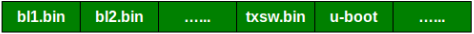
\includegraphics[width=\textwidth]{./data/images/odroid_boot_sequence.eps}
\caption{Odroid Boot Sequence}
\end{figure}

\begin{enumerate}
 \item iROM (Code inside the SoC) will attempt to read the boot media at the first 512 bytes of it. On those first 512 bytes fwbl1 should exist. fwbl1 is signed by Samsung.
 \item fwbl1 will load bl2 (SPL) that is part of the U-Boot. bl2 is signed by Hardkernel
 \item bl2 will load U-boot. U-Boot is signed by us. However, we still have no way to integrate this with the bl2 part.
 \item U-Boot will do whats left, such as handle TrustZone, load kernel image and Ramdisk.
\end{enumerate}

\noindent
\textbf{U-Boot Verified RSA Boot \tobetested{}}

U-Boot has support for booting signed linux kernel images. To enable it we need to define the following variables on U-Boot,

\begin{itemize}
 \item CONFIG\_FIT  enable support for the FIT uImage format
 \item CONFIG\_OF\_CONTROL, CONFIG\_OF\_SEPARATE enable FDT
 \item CONFI\_FIT\_SIGNATURE enables signature verification of FIT images
 \item CONFIG\_RSA enable the RSA algorithm used for FIT image verification
\end{itemize}


and then follow the steps as described at doc/uimage.FIT/* on the U-Boot repository. The kernel will be signed using our custom keys. To boot a signed kernel we need to use the Flat Image Tree (FIT) format provided by U-Boot. This needs to be implemented in a way that does not prohibit us to perform conditional booting (i.e. boot a kernel based on its data integrity; checksum)

\noindent
\textbf{Signed Kernel Modules \tested{}}

The Linux kernel support the signing of modules. This way only modules signed by us would be able to be loaded. See \url{http://wiki.gentoo.org/wiki/Signed_kernel_module_support}



\subsubsection{Application Execution}
\tested{}


The Linux kernel supports the extension of the i-nodes of the file system with hash value of the files and signing of the hash to provide integrity check for files.

In the case that there is a miss match between the stored and the computed hash access is denied to the file.

Linux-IMA (Integrity Measurement Architecture):
\begin{itemize}
 \item \url{http://sourceforge.net/p/linux-ima/wiki/Home/}
 \item \url{https://wiki.gentoo.org/wiki/Integrity_Measurement_Architecture}
 \item \url{http://researcher.watson.ibm.com/researcher/view_group.php?id=2851}
 \item \url{http://lwn.net/Articles/488906/}
 \item \url{http://sourceforge.net/p/linux-ima/wiki/Home/#compiling-the-kernel-with-evmima-appraisal-enabled}
\end{itemize}


IMA-EVM (Extended Verification Module) 
\begin{itemize}
 \item \url{https://wiki.gentoo.org/wiki/Extended_Verification_Module}
\end{itemize}


\subsubsection{Kernel Configuration}
Minimal kernel setup (all unneeded modules should be removed). This can help with preventing someone to attach a foreign unit.

\subsubsection{System Updates}

From the techniques described above we get a locked system that is hard to be altered by an attacker. However, a locked system can become outdated and thus easier to exploit. We need to find a secure way to update our system without compromising its security. 

New kernels should be signed with a constant key as this would reside inside the U-Boot. This may also be the case for the IMA scheme too as we probably do not want to update the sign values on every update.

\subsection{Data Integrity}

All communication is encrypted. Probably use symmetric encryption to reduce overhead.

We need to be able to verify the integrity of the data that are send on the cloud. Otherwise, a compromised control node or guest node can fill the storage with bogus data.

\subsection{Monitoring}

Eagle-eye view of the nodes. Reports on logins, permission denials, changes in important files, attempts of physical break.

See appendix A for monit

